\documentclass{article}

\usepackage[utf8]{inputenc}
\usepackage[T1]{fontenc}
\usepackage[greek,english]{babel}
\usepackage{alphabeta}
\usepackage{amsmath}
\usepackage{amssymb}
\usepackage{graphicx}
\usepackage{subcaption}
\usepackage{epstopdf}
\usepackage[margin=1in, paperwidth=7.5in,paperheight=10.5in]{geometry}
\usepackage{hyperref}
\usepackage{paracol}

\newcommand\course{TΗΛ411}
\newcommand\courseName{Ψηφιακή Επεξεργασία Εικόνας}
\newcommand\semester{Χειμερινό 2021}
\newcommand\assignmentNumber{Assignment 4}
\newcommand\studentName{Μαυρογιώργης Δημήτρης}                           
\newcommand\studentNumber{2016030016}

\title{\underline{\textbf{\assignmentNumber}}} 
\author{\textsc{\textbf{Όνομα:}}  \studentName\\
		\textsc{\textbf{ΑΜ:}}  \studentNumber\\
		\course \ - \courseName\\ 
		\textsc{Πολυτεχνείο Κρήτης}
}
\date{\today}
\begin{document}
	\maketitle

\section*{Introduction}
	Ο σκοπός της 4ης εργαστηριακής άσκησης είναι η δημιουργία τριών φίλτρων ενίσχυσης μιας εικόνας. Πιο συγκεκριμένα, έπρεπε να υλοποιήσουμε ένα φίλτρο της διαμέσου (median), ένα φίλτρο της μέγιστης τιμής (max) και ένα φίλτρο της ελαχιστης τιμής (min). Σκοπός ήταν να δημιουργήσουμε μία συνάρτηση, η οποία θα παίρνει ως όρισμα την αρχική εικόνα, το φίλτρο και το είδος του φίλτρου, και να επιστρέφει μια νέα εικόνα ίδιων διαστάσεων με την αρχική. 

\section*{Implementation}
	Για την υλοποίηση της συνάρτησης που τα εφαρμόζει ένα από τα τρία φίλτρα στην εικόνα, χρειάστηκε να συμπληρώσουμε κατάλληλο αριθμό σειρών και στηλών με μηδενικά με τη συνάρτηση padarray έτσι, ώστε να μπορέσει να εφαρμοστεί το φίλτρο στα άκρα της εικόνας. Ο αριθμός των σειρών και στηλών που συμπλρώνεται ανάλογα με το μέγεθος m του φίλτρου έιναι $\left \lfloor \frac{m}{2} \right \rfloor  $. \\
	
	\noindent
	Έπειτα από τη συμπήρωση, η διαδικασία που ακολουθούμε είναι να πάρουμε τα pixel μιας γειτονίας στην οποία εφαρμόζεται το φίλτρο, να ταξινομίσουμε τις τιμές των pixel και έπειτα να πάρουμε τη median, max ή min τιμή ανάλογα με το είδος του φίλτρου, που εφαρμόζουμε κάθε φορά. Αυτή τη διαδικάσία την εφαρμόζουμε για κάθε pixel της αρχικής εικόνας και το αποτέλεσμα που θα προκύψει είναι μία νέα εικόνα ίδιων διαστάεων με την αρχική.
	
\section*{Results}
	\subsubsection*{Median Filter}
	
	\noindent
	Όπως φαίνεται και στις εικόνες παρακάτω, η εφαρμογή του φίλτρου διαμέσου, βελτιώνει σε αρκετά μεγάλο βαθμό την εικόνα, αφαιρώντας το θόρυβο και εξομαλύνοντάς την. Πιο συγκεκριμένα, αυτο που παρατησρούμε είναι ότι ο θόρυβος εξαφανίζεται εντελώς,  καθώς αυξάνεται η διάσταση του φίλτρου. Ωστόσο, βλέπουμε ότι σε πολύ μεγάλες διαστάσεις, όπως πχ στην περίπτωση του 9x9 φίλτρου, ναι με γίνεται η αποθορυβοποίηση και εξομάλυνση της εικόνας, αλλα χειροτερεύει η ανάλυσή της. Επιπλέον, στην περίπτωση που η εικόνα έχει περισσότερο θόρυβο βλέπουμε ότι για τις δεδομένες διαστάσεις φιλτρων, δεν γίνεται πλήρης αποθορυβοποίηση της εικόνας, αλλά υπάρχει μεγάλη βελτίωση σε σχέση με την αρχική εικόνα.
	
	\pagebreak
	\begin{figure}[h!]
			\centering
			\begin{subfigure}[t]{0.5\textwidth}
				\centering
				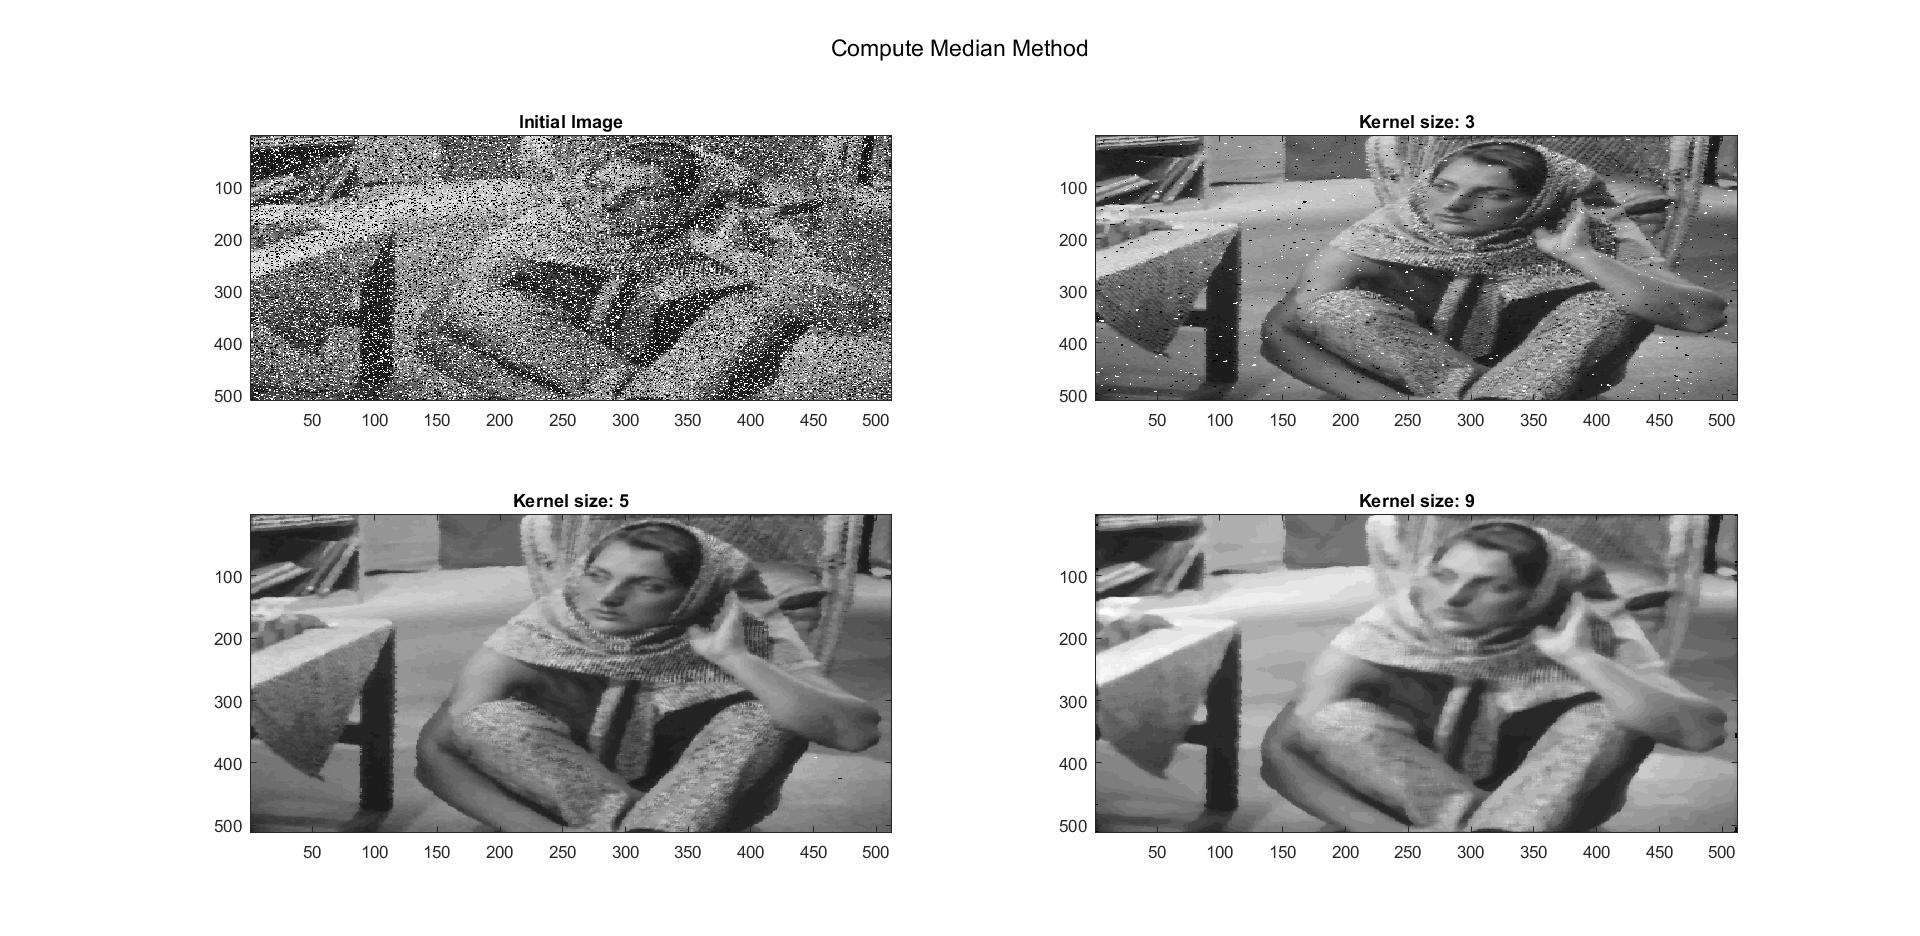
\includegraphics[height=\linewidth, width=\linewidth]{./output_images/img_noisy_1_median.jpg}
			\end{subfigure}%
			~
			\begin{subfigure}[t]{0.5\textwidth}
				\centering
				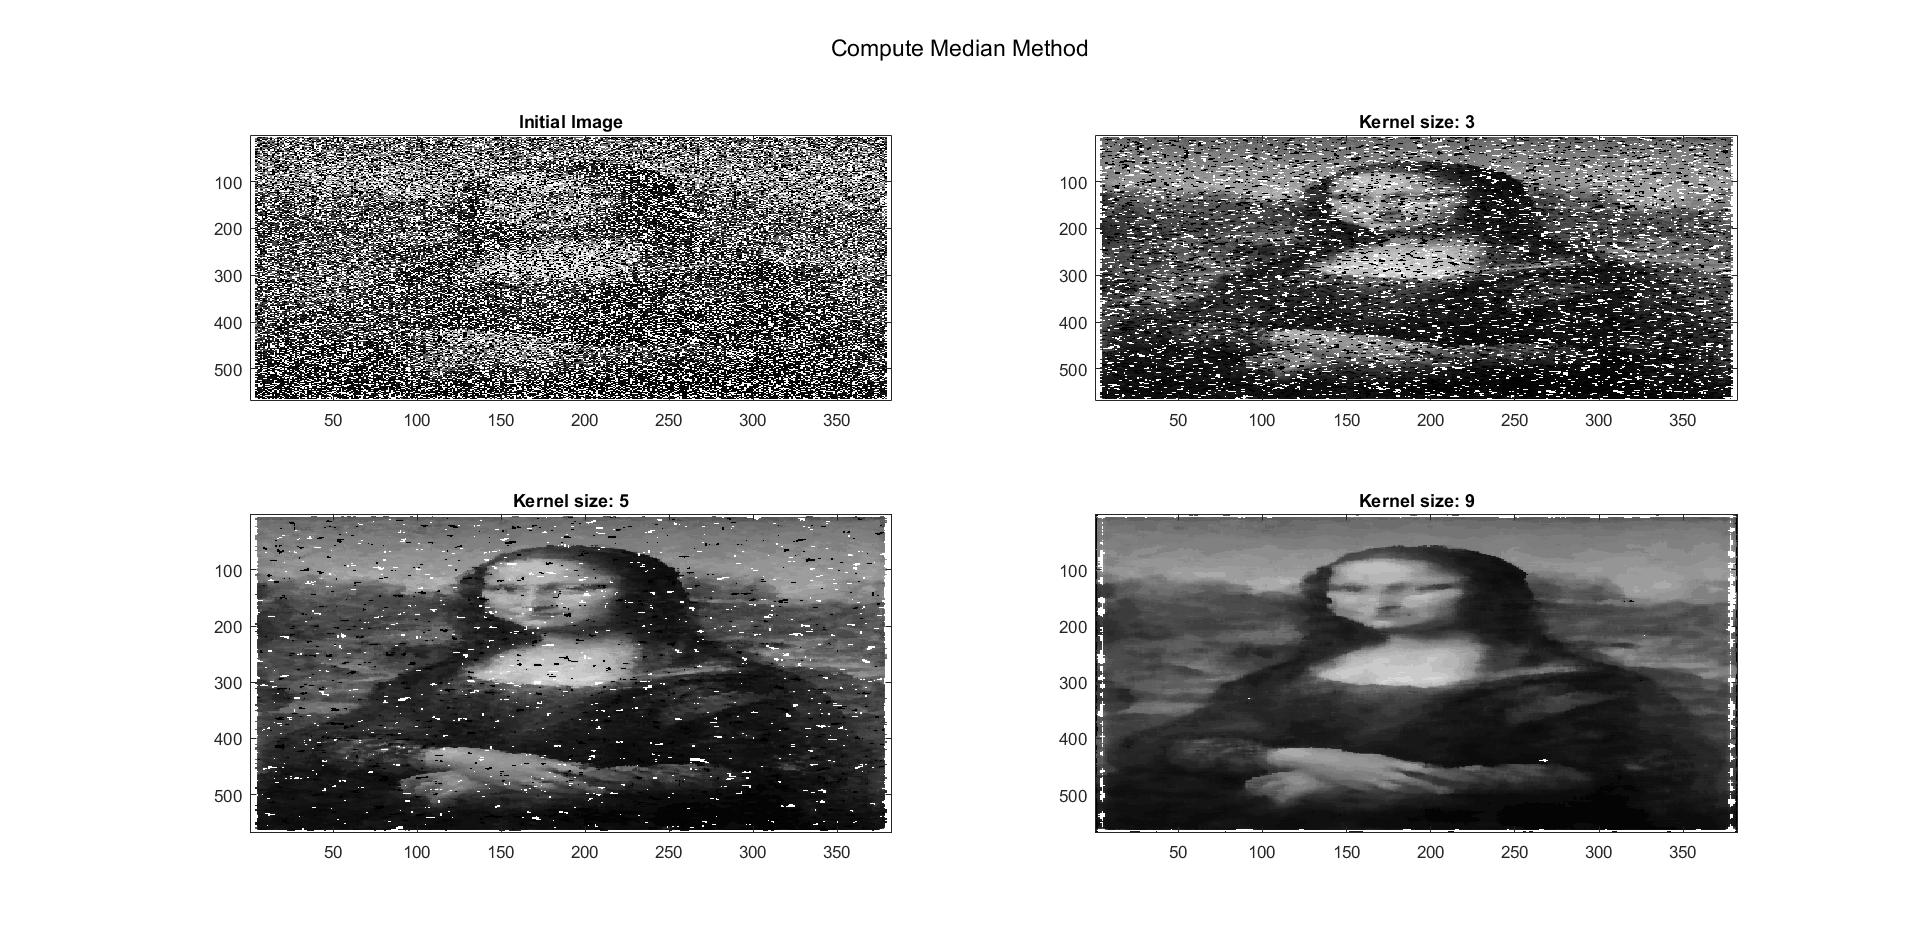
\includegraphics[height=\linewidth, width=\linewidth]{./output_images/img_noisy_2_median.jpg}
			\end{subfigure}	
			\caption{Application of 3x3, 5x5 and 9x9 Median filter to two different noisy images}
		\end{figure}

\subsubsection*{Max Filter}
	Σε αυτή την περίπτωση εφαρμογής του max φίλτρου, βλέπουμε ότι ο θόρυβος αντί να εξαφανίζεται, αυξάνεται, με αποτέλεσμα να χάνεται η πληροφορία της εικόνας. Ειδικότερα, και στις δύο περιπτώσεις, παρατηρούμε ότι με την αύξηση της διάστασης του φίλτρου τα αποτελέσματα γίνονται χειρότερα και δε βελτιώνεται η εικόνα, επειδή το φίλτρο επιλέγει τη μέγιστη τιμή μιας γειτονιάς και έτσι οι τιμές των pixel της τελικής εικόνας να είναι πιο κοντά στο γκρι προς λευκό τόνο.\\
	
	\begin{figure}[h!]
		\centering
		\begin{subfigure}[t]{0.5\textwidth}
			\centering
			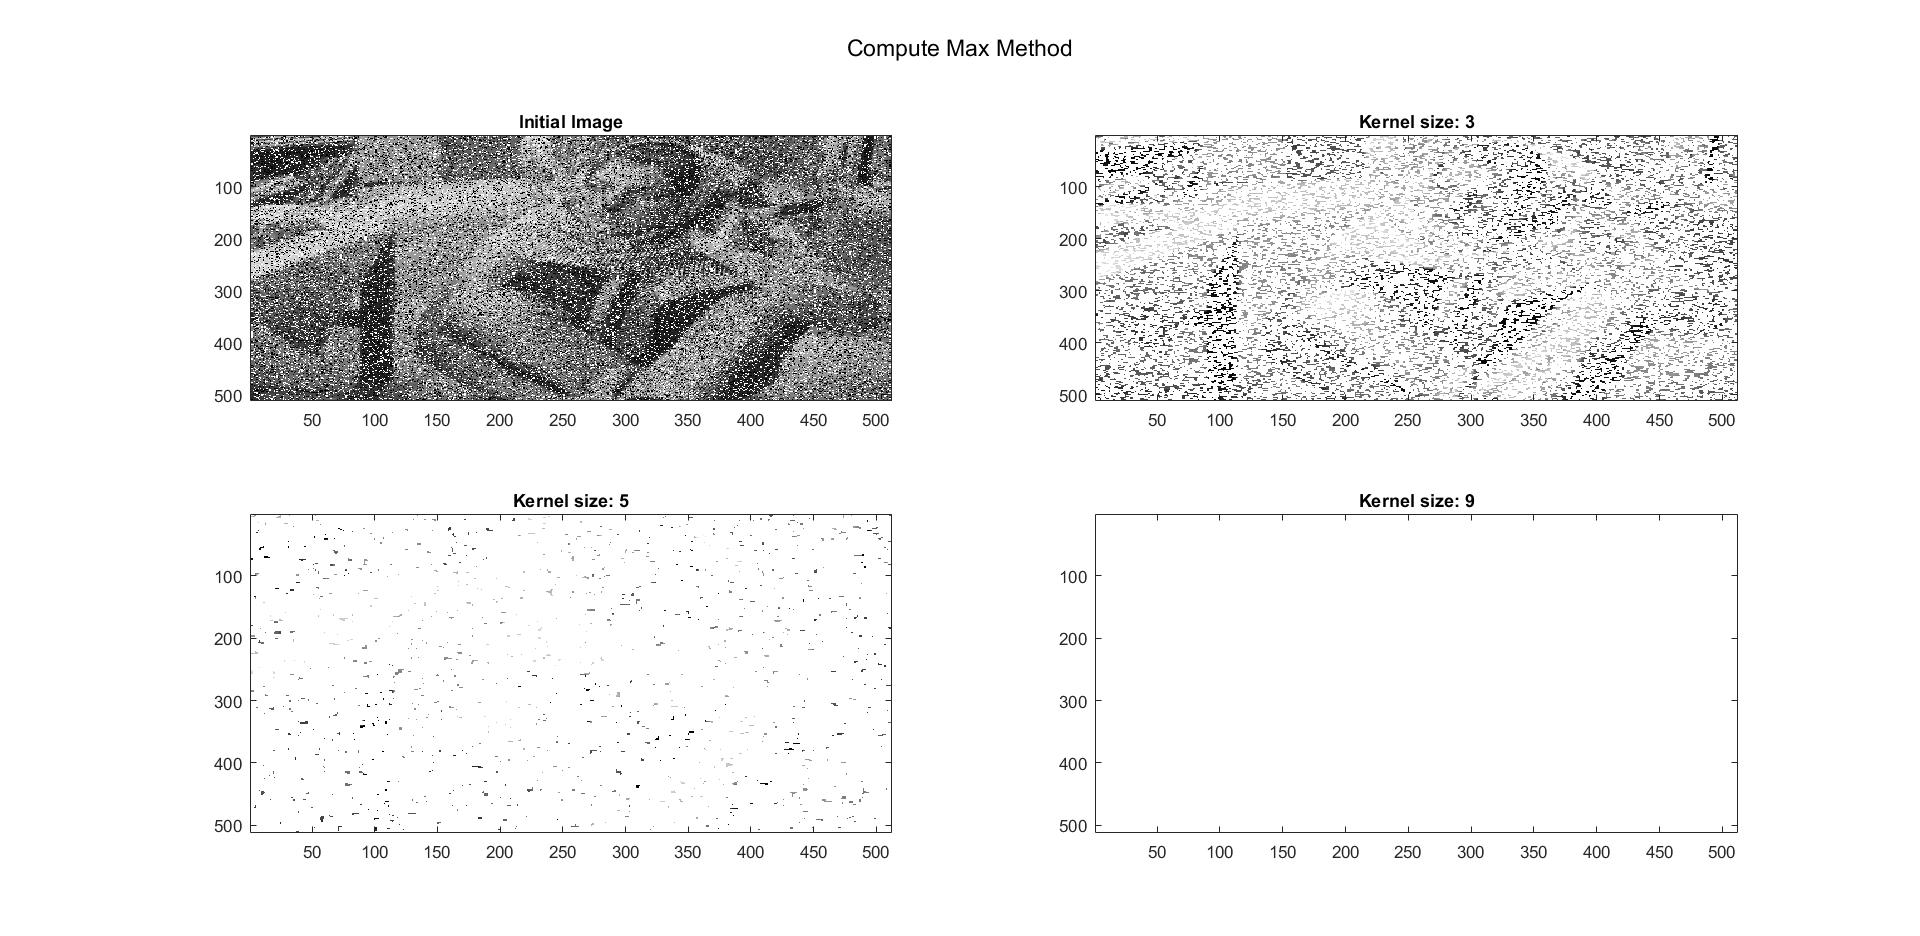
\includegraphics[height=\linewidth, width=\linewidth]{./output_images/img_noisy_1_max.jpg}
		\end{subfigure}%
		~
		\begin{subfigure}[t]{0.5\textwidth}
			\centering
			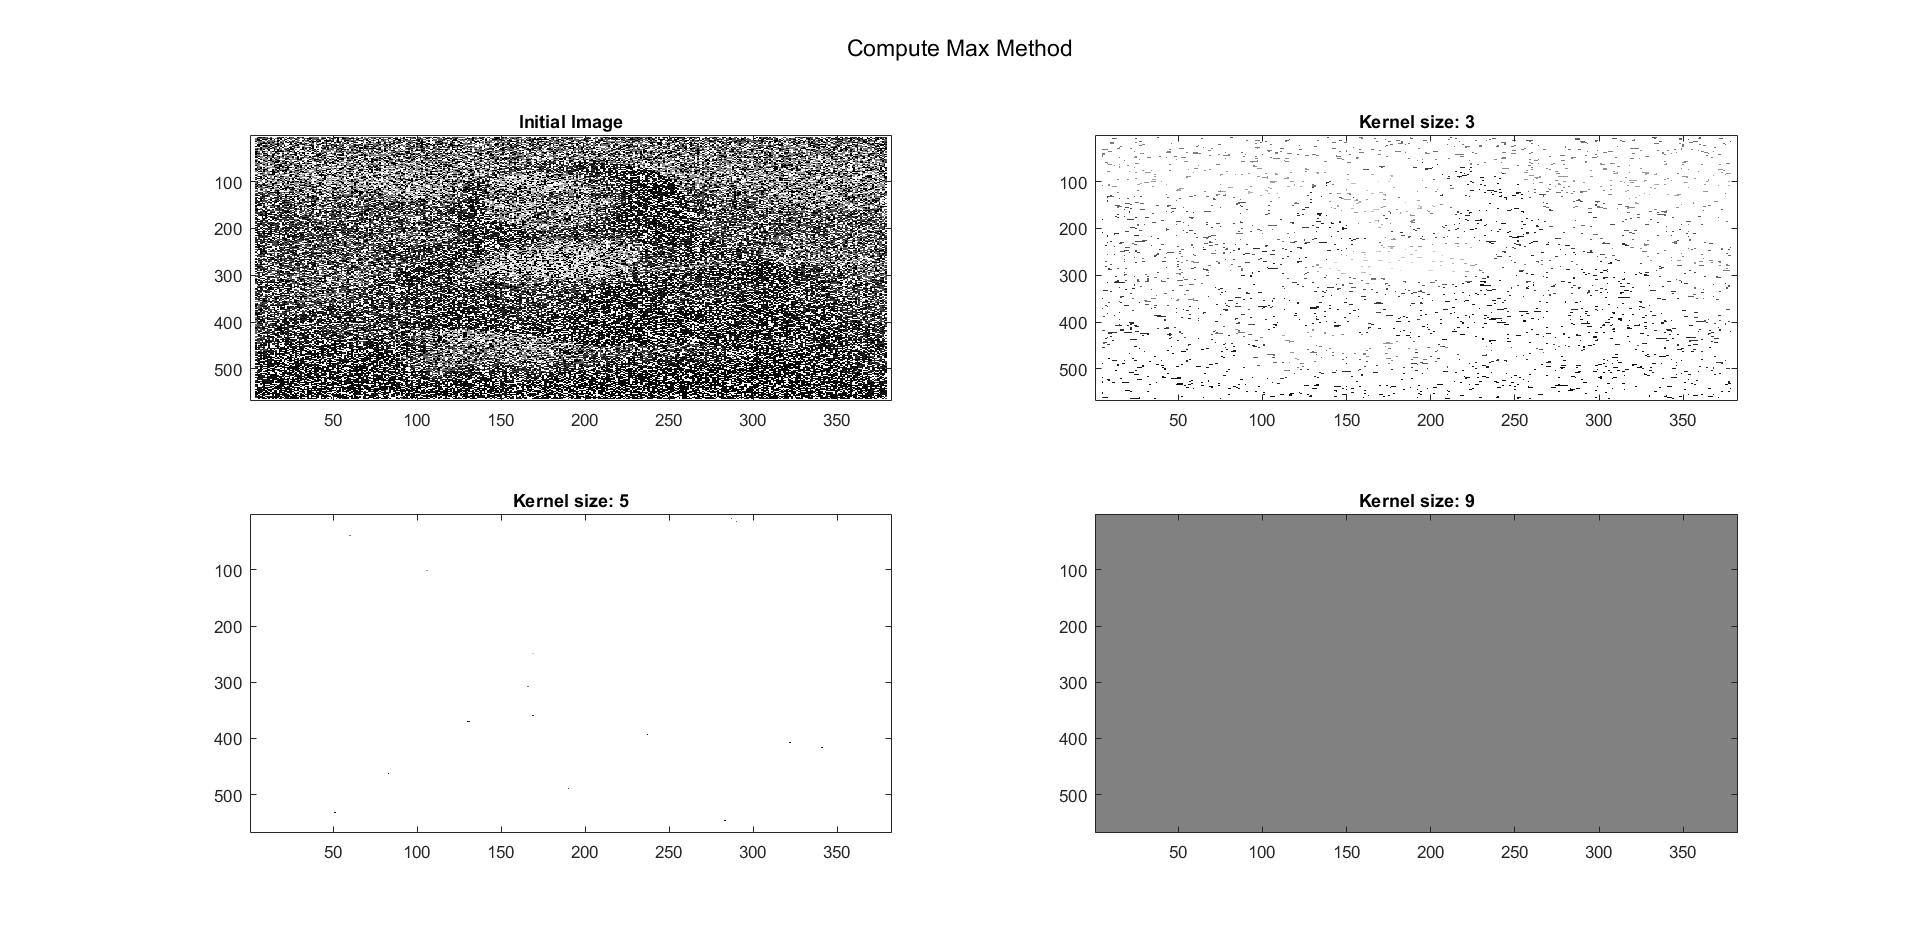
\includegraphics[height=\linewidth, width=\linewidth]{./output_images/img_noisy_2_max.jpg}
		\end{subfigure}	
		\caption{Application of 3x3, 5x5 and 9x9 Max filter to two different noisy images}
	\end{figure}
	
\pagebreak
\subsubsection*{Min Filter}
	Τέλος, στην περίπτωση εφαρμογής του min φίλτρου, βλέπουμε ότι επίσης ο θόρυβος δεν εξαφανίζεται, με αποτέλεσμα να χάνεται και σε αυτή την περίπτωση η πληροφορία της εικόνας. Ειδικότερα, παρατηρούμε ότι με την αύξηση της διάστασης του φίλτρου τα χειροτερεύουν, με αποτέλεσμα να μη βελτιώνεται η εικόνα. Αντίθετα, με την περίπτωση του max, εδώ οι τιμές των pixel μετά την εφαρμογή του φίλτρου είναι πιο κοντά στο μαύρο τόνο.\\
	
	\begin{figure}[h!]
		\centering
		\begin{subfigure}[t]{0.5\textwidth}
			\centering
			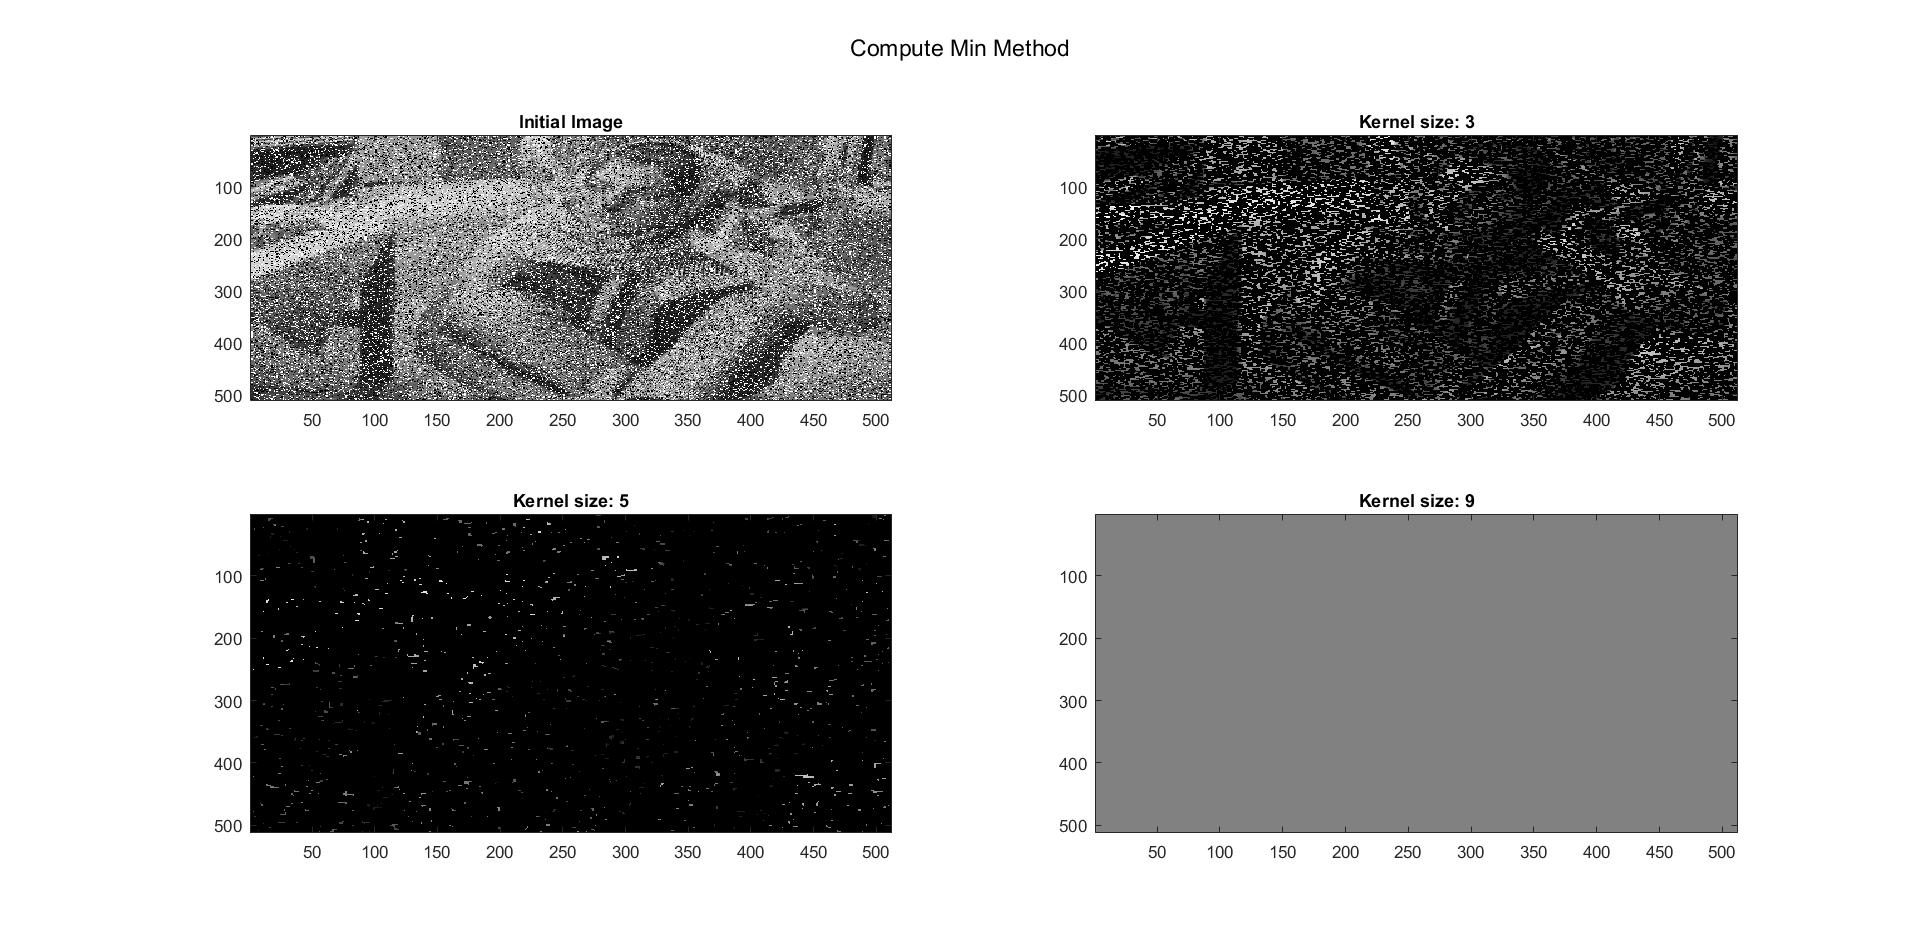
\includegraphics[height=\linewidth, width=\linewidth]{./output_images/img_noisy_1_min.jpg}
		\end{subfigure}%
		~
		\begin{subfigure}[t]{0.5\textwidth}
			\centering
			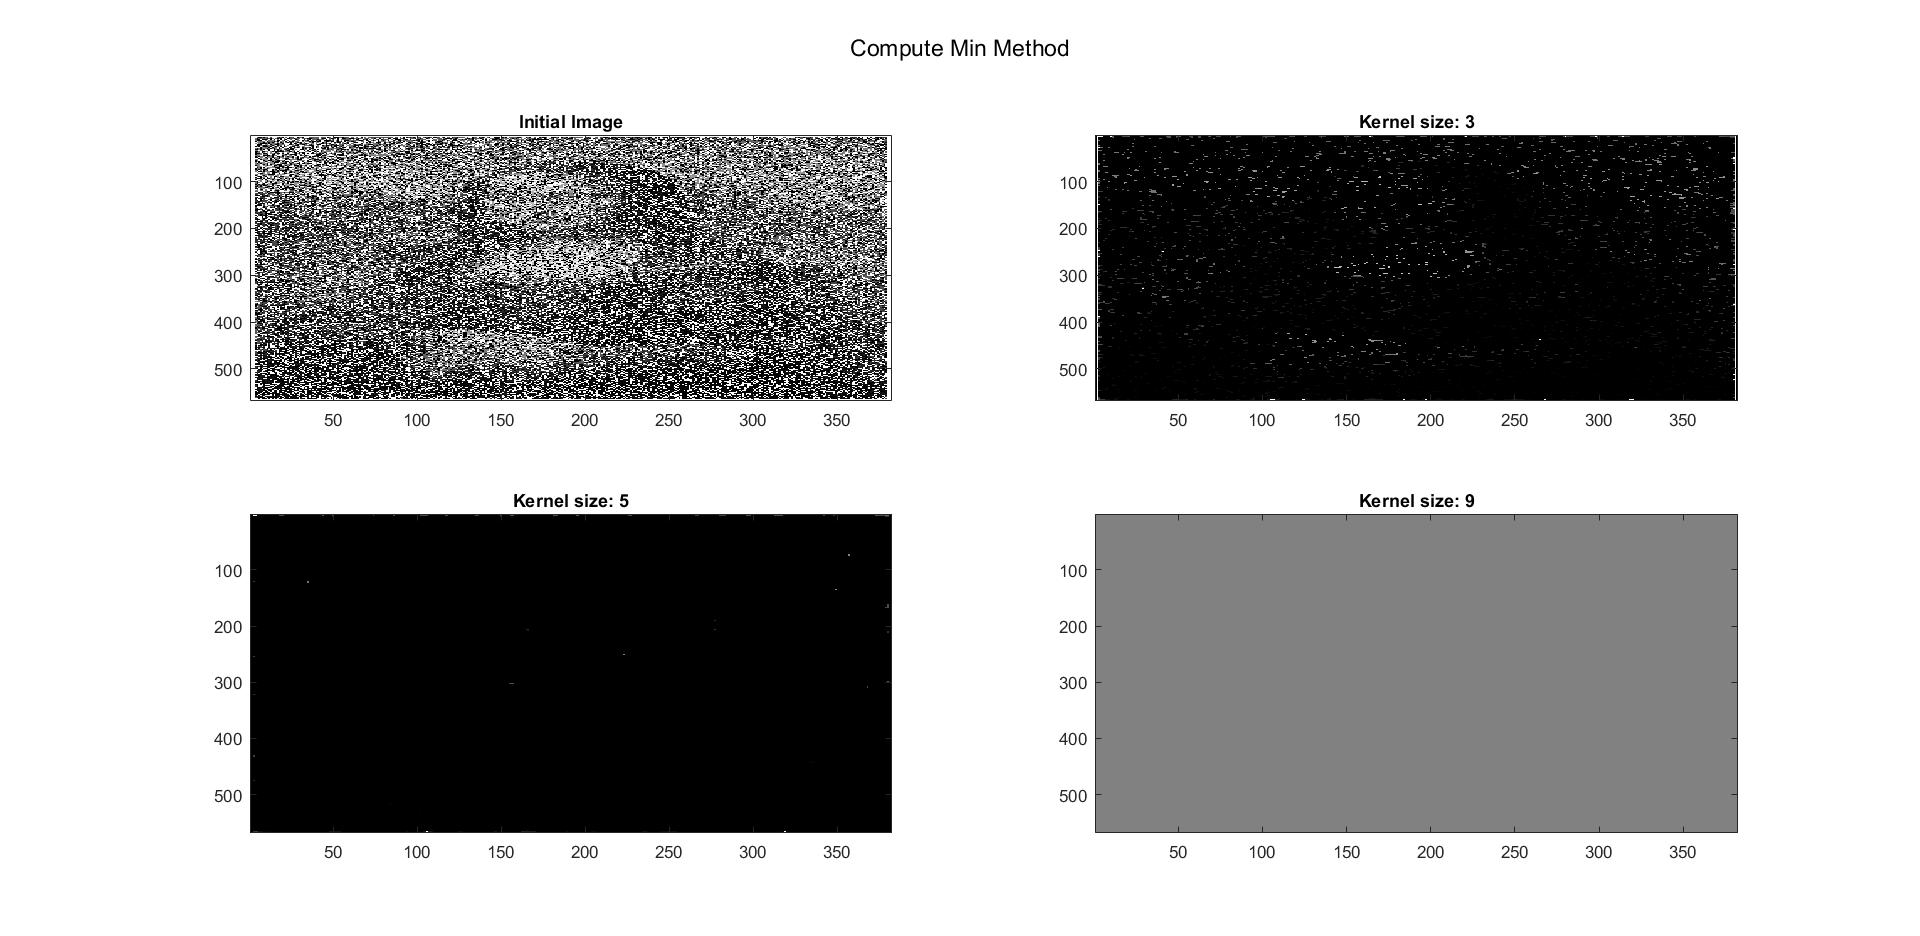
\includegraphics[height=\linewidth, width=\linewidth]{./output_images/img_noisy_2_min.jpg}
		\end{subfigure}	
		\caption{Application of 3x3, 5x5 and 9x9 Min filter to two different noisy images}
	\end{figure}
	
	\subsubsection*{Bonus Εxercise}
		Για την εφαρμογή του διαφορικού φίλτρου F = [-1 0 1], κάνουμε πρώτα τη συνέλιξη του φίλτρου F με τις γραμμές της εικόνας Ι. Έπειτα, θα πρέπει να κάνουμε τη συνέλιξη του φίλτρου $F^{T}$ (περιστροφή κατά $90^{ο}$) με τις στήλες της εικόνας Ι. Τέλος, αθροίζουμε τις δύο συνελίξεις για να πάρουμε το επιθυμητό αποτέλεσμα. Μετά από αυτή τη διαδικάσία εξάγουμε τις ακμές μιας εικόνας και τα αποτελέσματα φαινονται στο παρακάτω figure.
		\begin{figure}[h!]
			\centering
			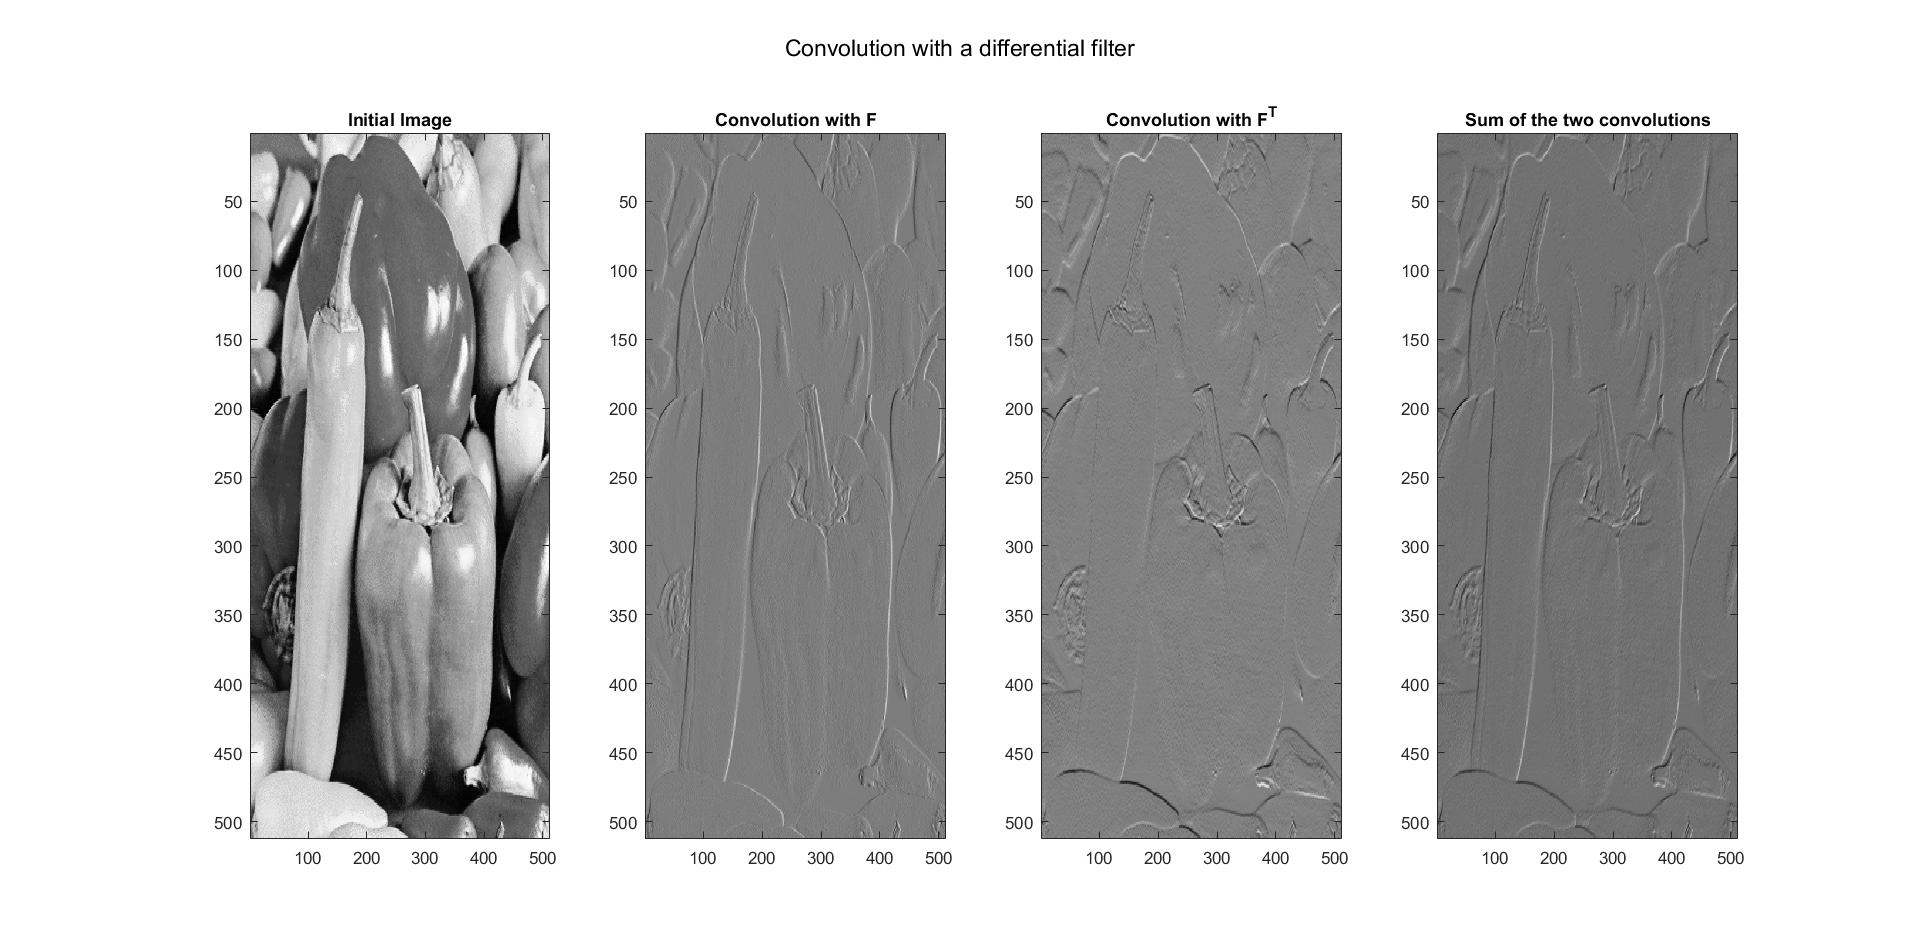
\includegraphics[height=0.35\linewidth, width=\linewidth]{./output_images/img_peppers_dif_filter.jpg}
			\caption{Application of 3x1 differential filter to pepers image}
		\end{figure}
\end{document}
